\section{Arbre binaire}

Le labyrinthe est une simple matrice où chaque élément est une \textit{Case}. Mais on peut aussi le décomposer en un arbre binaire car le labyrinthe imposé dans le projet est dit "parfait" \footnote{Cette notion a été reprise de $\href{http://fr.wikipedia.org/wiki/Mod\%C3\%A9lisation_math\%C3\%A9matique_d\%27un_labyrinthe}{fr.wikipedia}$.}.

\begin{figure}[!h]
  \centering
  \subfloat[Un labyrinthe parfait contenant son arbre.]{\label{fig:edge-a}
\includegraphics[width=0.4\textwidth]{4.arbreBinaire/maze.pdf}}
  \hspace{5pt}
  \subfloat[Représentation en arbre du labyrinthe.]{\label{fig:contour-b}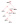
\includegraphics[width=0.4\textwidth]{4.arbreBinaire/tree.pdf}}
  \hspace{5pt}
  \caption{Le labyrinthe et son arbre associé.}
\end{figure}

Cette arbre est donc construit par la classe \textit{Path} sous forme de plusieurs \textit{Tree} comme vu au cours.